% CVPR 2026 Paper Template; see https://github.com/cvpr-org/author-kit

\documentclass[10pt,twocolumn,letterpaper]{article}

%%%%%%%%% PAPER TYPE  - PLEASE UPDATE FOR FINAL VERSION
% \usepackage{cvpr}              % To produce the CAMERA-READY version
% \usepackage[review]{cvpr}      % To produce the REVIEW version
\usepackage[pagenumbers]{cvpr}
\usepackage{tikz}
\usetikzlibrary{positioning, shapes.geometric, arrows.meta, calc}
\usepackage{CJKutf8}
% \usepackage[pagenumbers]{cvpr} % To force page numbers, e.g. for an arXiv version

% Import additional packages in the preamble file, before hyperref
\input{preamble}

% It is strongly recommended to use hyperref, especially for the review version.
% hyperref with option pagebackref eases the reviewers' job.
% Please disable hyperref *only* if you encounter grave issues, 
% e.g. with the file validation for the camera-ready version.
%
% If you comment hyperref and then uncomment it, you should delete *.aux before re-running LaTeX.
% (Or just hit 'q' on the first LaTeX run, let it finish, and you should be clear).
\definecolor{cvprblue}{rgb}{0.21,0.49,0.74}
\usepackage[pagebackref,breaklinks,colorlinks,allcolors=cvprblue]{hyperref}

%%%%%%%%% PAPER ID  - PLEASE UPDATE
\def\paperID{*****} % *** Enter the Paper ID here
\def\confName{CVPR}
\def\confYear{2026}

%%%%%%%%% TITLE - PLEASE UPDATE
\title{Introduction to Machine Learning Final Projects\\Titanic: Machine Learning from Disaster}

%%%%%%%%% AUTHORS - PLEASE UPDATE
\author{鍾承翰\\
112550189\\
{\small Contributions:}\\
{\small Code Writing, Report 34\%}
\and
陳景寬\\
112550112\\
{\small Contributions:}\\
{\small Slides, Video Recording 33\%}
\and
林昌岳\\
113511248\\
{\small Contributions:}\\
{\small Slides, Video Recording 33\%}
}

\begin{document}
\begin{CJK*}{UTF8}{bsmi}
\maketitle
\begin{abstract}
We investigate feature engineering strategies for Titanic survival prediction through systematic comparison of three pipelines: RF (community practices), XGB (gradient boosting optimized), and MLP (neural network ready). Testing seven algorithms across multiple random seeds, we find that thoughtful feature construction—particularly title extraction and family size derivation—matters more than model complexity. Our Random Forest with RF features achieves 79.67\% accuracy, ranking top 8\% on Kaggle. Results demonstrate that domain-informed feature engineering remains crucial for small tabular datasets, where tree-based methods outperform neural networks without extensive tuning.
\end{abstract}

\section{Introduction}
\label{sec:introduction}

\subsection{Problem Background}

The sinking of the RMS Titanic on its maiden voyage represents not only a historical tragedy but also a rich data source for understanding survival patterns under extreme circumstances. The Kaggle competition "Titanic: Machine Learning from Disaster" challenges participants to predict passenger survival based on demographic and ticketing information. With 891 training samples and 418 test samples, each described by features including passenger class (Pclass), name, sex, age, number of siblings/spouses aboard (SibSp), number of parents/children aboard (Parch), ticket number, fare, cabin, and port of embarkation (Embarked), the dataset presents a classic binary classification task with realistic complications: missing values, categorical variables, and potential non-linear interactions between features.

The survival rate in the training set is approximately 38\%, indicating moderate class imbalance. Initial exploratory analysis reveals strong predictive signals: women and children had significantly higher survival rates due to the "women and children first" evacuation protocol, first-class passengers enjoyed better access to lifeboats, and fare prices correlated with both passenger class and survival likelihood. However, raw features alone provide insufficient discriminative power—sophisticated feature engineering is required to extract latent information encoded in passenger names (social titles), ticket numbers (group bookings), and cabin assignments (deck locations).

% INSERT FIGURE 1: Survival by Gender and Class
\begin{figure}[t]
    \centering
    \includegraphics[width=0.48\columnwidth]{figures/survival_by_sex.png}
    \includegraphics[width=0.48\columnwidth]{figures/survival_by_pclass.png}
    \caption{Exploratory analysis of survival patterns: (left) survival rate by gender showing strong bias toward female passengers (74.2\% vs 18.9\%); (right) survival rate by passenger class demonstrating socioeconomic advantage (63.0\% first class vs 24.2\% third class).}
    \label{fig:survival_patterns}
\end{figure}

% INSERT FIGURE 2: Age Distribution
\begin{figure}[t]
    \centering
    \includegraphics[width=0.95\columnwidth]{figures/age_distribution.png}
    \caption{Age distribution of passengers by survival status. Survivors show a slightly younger mean age (28.3 years) compared to non-survivors (30.6 years), with notable representation of children under 12 among survivors.}
    \label{fig:age_dist}
\end{figure}

\subsection{Our Approach}

In this work, we conduct a systematic investigation of feature engineering strategies and model selection for Titanic survival prediction. Our contributions are as follows:

\textbf{1. Comprehensive Feature Engineering Comparison:} We implement and compare three distinct feature engineering pipelines:
\begin{itemize}
    \item \textbf{RF (Random Forest-oriented):} Based on community best practices, featuring title simplification (Mr, Mrs, Miss, Master, Rare), family size aggregation, ticket prefix extraction, and cabin deck identification. Missing ages are imputed using a Random Forest regressor trained on available demographic features.
    \item \textbf{XGB (XGBoost-optimized):} Incorporates frequency encoding for high-cardinality categorical variables (ticket types, cabin assignments), interaction terms (Sex×Pclass, Pclass×AgeBin), and quartile-based fare binning to capture non-linear pricing effects.
    \item \textbf{MLP (Neural Network-ready):} Employs one-hot encoding for all categorical features with \texttt{drop\_first=True} to avoid multicollinearity, standardized continuous variables via StandardScaler, and carefully designed binning strategies for age and fare to assist gradient-based optimization.
\end{itemize}

\textbf{2. Rigorous Multi-Model Evaluation:} We train and evaluate six classical machine learning algorithms (Random Forest, Gradient Boosting, XGBoost, Logistic Regression, SVM, KNN) and one neural network (MLP) using consistent train-validation splits with stratified sampling. For tree-based methods, we perform grid search over key hyperparameters (number of estimators, learning rate, max depth, subsample ratio). For distance-based methods (SVM, KNN), we incorporate feature scaling within scikit-learn pipelines. All experiments are repeated across multiple random seeds (45, 2025, 777) to assess prediction stability and variance.

Our experimental results demonstrate that feature engineering choice has a more pronounced impact on performance than algorithmic selection within reasonable model families. The RF feature set paired with Random Forest classifier achieves the highest single-model validation accuracy of 79.67\%. Ablation studies reveal that title extraction and family size features contribute most significantly to predictive power, followed by strategic age imputation.
\section{Code Description}
\label{sec:code}

This section provides a detailed technical description of our implementation, covering the project architecture, feature engineering pipelines, model configurations, and training procedures. The complete codebase is organized into modular components to facilitate reproducibility and extensibility.

\subsection{Project Architecture}

The project follows a clean, modular design pattern with clear separation of concerns. Figure~\ref{fig:system_architecture} illustrates the complete system architecture and data flow. The main components are:

% INSERT FIGURE: System Architecture
% System Architecture Diagram - Simplified and Cleaner Version
% Add this to your Code Description section

\begin{figure*}[t]
    \centering
    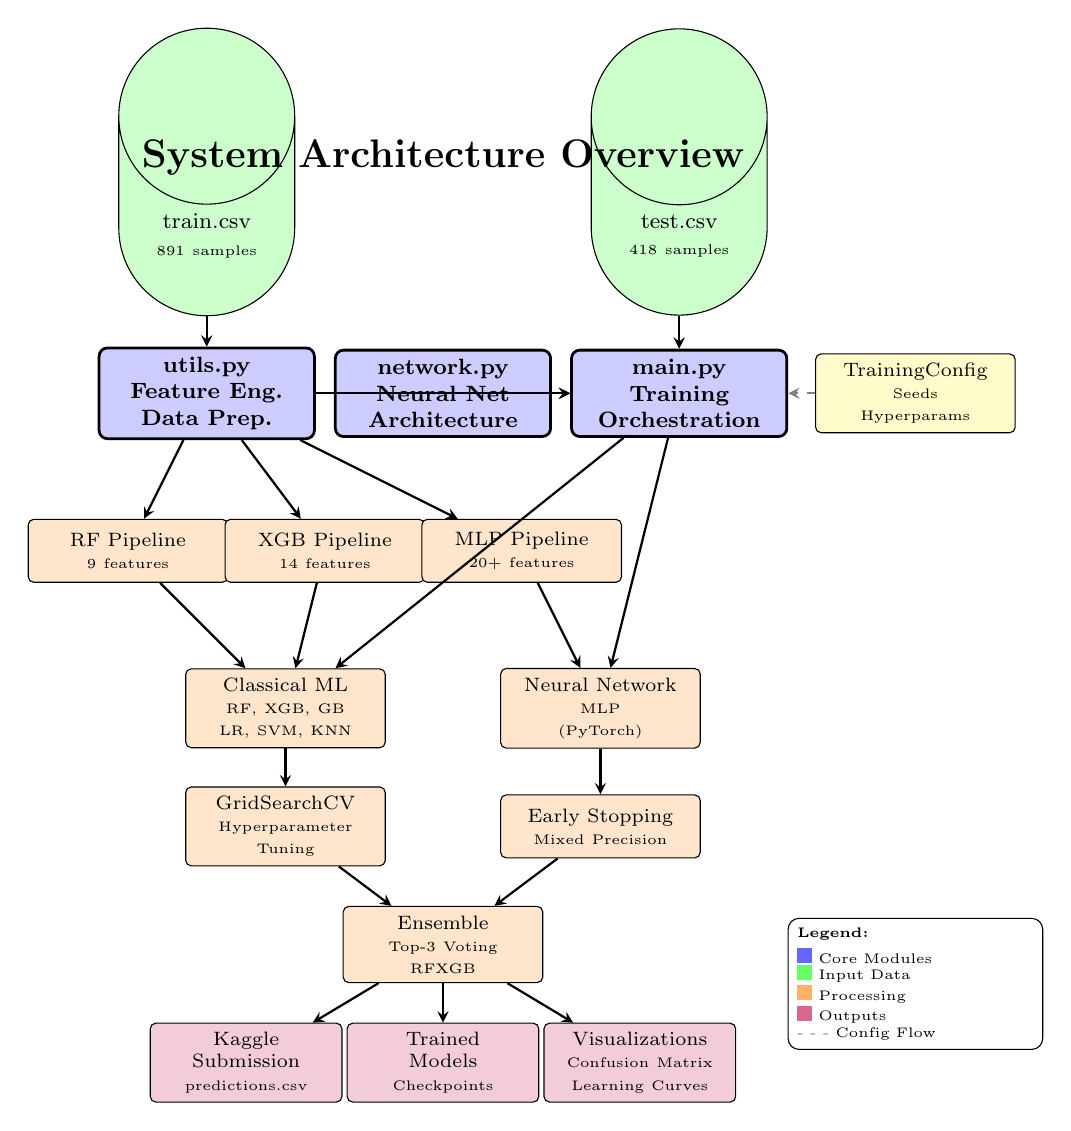
\begin{tikzpicture}[
        node distance=1.5cm and 2cm,
        module/.style={rectangle, draw, fill=blue!20, text width=2.5cm, align=center, minimum height=1cm, rounded corners=3pt, font=\footnotesize\bfseries, line width=1pt},
        data/.style={cylinder, draw, fill=green!20, text width=2cm, align=center, minimum height=0.8cm, shape border rotate=90, font=\footnotesize},
        process/.style={rectangle, draw, fill=orange!20, text width=2.3cm, align=center, minimum height=0.8cm, rounded corners=2pt, font=\scriptsize},
        output/.style={rectangle, draw, fill=purple!20, text width=2.2cm, align=center, minimum height=0.8cm, rounded corners=2pt, font=\scriptsize},
        arrow/.style={->, >=stealth, thick},
        dasharrow/.style={->, >=stealth, thick, dashed, gray}
    ]
    
    % Top: Data sources
    \node[data] (train) at (-3, 6) {train.csv\\{\tiny 891 samples}};
    \node[data] (test) at (3, 6) {test.csv\\{\tiny 418 samples}};
    
    % Layer 1: Core modules
    \node[module] (utils) at (-3, 4) {utils.py\\Feature Eng.\\Data Prep.};
    \node[module] (network) at (0, 4) {network.py\\Neural Net\\Architecture};
    \node[module] (main) at (3, 4) {main.py\\Training\\Orchestration};
    
    % Layer 2: Feature pipelines (simplified)
    \node[process] (rf) at (-4, 2) {RF Pipeline\\{\tiny 9 features}};
    \node[process] (xgb) at (-1.5, 2) {XGB Pipeline\\{\tiny 14 features}};
    \node[process] (mlp) at (1, 2) {MLP Pipeline\\{\tiny 20+ features}};
    
    % Layer 3: Model training
    \node[process] (classical) at (-2, 0) {Classical ML\\{\tiny RF, XGB, GB}\\{\tiny LR, SVM, KNN}};
    \node[process] (neural) at (2, 0) {Neural Network\\{\tiny MLP}\\{\tiny (PyTorch)}};
    
    % Layer 4: Tuning
    \node[process] (grid) at (-2, -1.5) {GridSearchCV\\{\tiny Hyperparameter}\\{\tiny Tuning}};
    \node[process] (early) at (2, -1.5) {Early Stopping\\{\tiny Mixed Precision}};
    
    % Layer 5: Ensemble
    \node[process] (ensemble) at (0, -3) {Ensemble\\{\tiny Top-3 Voting}\\{\tiny RFXGB}};
    
    % Layer 6: Outputs
    \node[output] (submission) at (-2.5, -4.5) {Kaggle\\Submission\\{\tiny predictions.csv}};
    \node[output] (models) at (0, -4.5) {Trained\\Models\\{\tiny Checkpoints}};
    \node[output] (viz) at (2.5, -4.5) {Visualizations\\{\tiny Confusion Matrix}\\{\tiny Learning Curves}};
    
    % Arrows: Data to modules
    \draw[arrow] (train) -- (utils);
    \draw[arrow] (test) -- (main);
    
    % Module connections
    \draw[arrow] (utils) -- (main);
    \draw[arrow] (network) -- (main);
    
    % Feature engineering to pipelines
    \draw[arrow] (utils) -- (rf);
    \draw[arrow] (utils) -- (xgb);
    \draw[arrow] (utils) -- (mlp);
    
    % Pipelines to models
    \draw[arrow] (rf) -- (classical);
    \draw[arrow] (xgb) -- (classical);
    \draw[arrow] (mlp) -- (neural);
    
    % Training flow
    \draw[arrow] (main) -- (classical);
    \draw[arrow] (main) -- (neural);
    
    % Tuning
    \draw[arrow] (classical) -- (grid);
    \draw[arrow] (neural) -- (early);
    
    % To ensemble
    \draw[arrow] (grid) -- (ensemble);
    \draw[arrow] (early) -- (ensemble);
    
    % Final outputs
    \draw[arrow] (ensemble) -- (submission);
    \draw[arrow] (ensemble) -- (models);
    \draw[arrow] (ensemble) -- (viz);
    
    % Configuration (top right)
    \node[process, fill=yellow!20] (config) at (6, 4) {TrainingConfig\\{\tiny Seeds}\\{\tiny Hyperparams}};
    \draw[dasharrow] (config) -- (main);
    
    % Title
    \node[font=\Large\bfseries] at (0, 7) {System Architecture Overview};
    
    % Legend (bottom right)
    \node[font=\tiny, text width=3cm, align=left, draw, fill=white, rounded corners] at (6, -3.5) {
        \textbf{Legend:}\\[2pt]
        \textcolor{blue!60}{\rule{0.8em}{0.8em}} Core Modules\\
        \textcolor{green!60}{\rule{0.8em}{0.8em}} Input Data\\
        \textcolor{orange!60}{\rule{0.8em}{0.8em}} Processing\\
        \textcolor{purple!60}{\rule{0.8em}{0.8em}} Outputs\\
        \textcolor{gray}{- - -} Config Flow
    };
    
    \end{tikzpicture}
    \caption{System architecture showing data flow from raw CSV files through feature engineering pipelines to model training and final predictions. The modular design separates data preparation (utils.py), neural network definitions (network.py), and training orchestration (main.py).}
    \label{fig:system_architecture}
\end{figure*}

\begin{itemize}
    \item \textbf{utils.py}: Core utilities including feature engineering functions, data preprocessing, configuration management, and custom PyTorch Dataset classes. Contains three distinct feature engineering pipelines: \texttt{\_engineer\_features\_rf()}, \texttt{\_engineer\_features\_xgb()}, and \texttt{\_engineer\_features\_mlp()}.
    
    \item \textbf{network.py}: Neural network architecture definition (TitanicMLP), training loop implementation with mixed precision support, evaluation functions, and inference utilities for test set predictions.
    
    \item \textbf{main.py}: Orchestration script that coordinates data loading, model training across multiple seeds, hyperparameter tuning via GridSearchCV, ensemble construction, and Kaggle submission generation.
\end{itemize}

Global configurations are centralized in \texttt{utils.py} through the \texttt{TrainingConfig} dataclass and module-level constants:

\begin{verbatim}
@dataclass(frozen=True)
class TrainingConfig:
    batch_size: int = 128
    num_epochs: int = 250
    learning_rate: float = 1e-3
    weight_decay: float = 1e-4
    val_ratio: float = 0.2
    patience: int = 30
    seed: int = 45
    seeds: tuple[int, ...] = (45, 2025, 777)
\end{verbatim}

This design allows easy experimentation with different hyperparameters and random seeds while maintaining consistency across runs.

\subsection{Feature Engineering Pipelines}

\subsubsection{RF Pipeline: Community Best Practices}

The RF feature engineering pipeline, adapted from Kaggle community solutions~\cite{elvennote2024titanic}, prioritizes interpretability and compatibility with tree-based methods. Key transformations include:

\textbf{Title Extraction and Simplification:} Passenger names follow the format ``Surname, Title. Firstname''. We extract titles using regex pattern matching and apply consolidation rules:
\begin{small}
\begin{verbatim}
# Extract title from name using regex
titles = name.str.extract(' ([A-Za-z]+)\.', 
                          expand=False)
# Consolidate rare titles
titles = titles.replace({
    'Mlle': 'Miss', 'Ms': 'Miss', 
    'Mme': 'Mrs', 'Dr': 'Mr', 
    'Major': 'Mr', 'Col': 'Mr'
})
\end{verbatim}
\end{small}
This reduces title cardinality from 17 unique values to 5 meaningful categories (Mr, Mrs, Miss, Master, Rare), capturing social status and age group signals.

\textbf{Ticket Prefix Processing:} Ticket numbers often contain alphanumeric prefixes indicating group bookings or special fare classes. We extract prefixes by removing punctuation and taking the first token:
\begin{verbatim}
ticket_prefix = ticket.replace('.', '')
                      .replace('/', '')
                      .strip().split(' ')[0]
\end{verbatim}
Purely numeric tickets are assigned a special marker "X".

\textbf{Age Imputation via RandomForest:} Missing ages (19.9\% of training data) are imputed using a RandomForestRegressor with 2000 trees, trained on non-missing samples after removing outliers (values beyond 4 standard deviations in Fare or Family\_Size):
\begin{small}
\begin{verbatim}
# Train RF regressor for age imputation
rf_model = RandomForestRegressor(
    n_estimators=2000, 
    random_state=42
)
rf_model.fit(age_train[age_features], 
             age_train['Age'])

# Predict missing ages
imputed = rf_model.predict(age_null_rows)
\end{verbatim}
\end{small}
This non-parametric approach captures complex interactions between age and other features (Pclass, Sex, Title, Fare) without assuming linearity.

\textbf{Categorical Encoding:} All categorical features (Sex, Embarked, Pclass, Title, Cabin, Ticket\_info) are converted to integer codes via pandas category dtype. This encoding is efficient for tree-based models but may not preserve ordinal relationships.

The final RF feature set consists of 9 features: Age, Embarked, Fare, Pclass, Sex, Family\_Size, Title2, Ticket\_info, and Cabin.

\subsubsection{XGB Pipeline: Gradient Boosting Optimization}

The XGB pipeline extends the RF approach with techniques specifically beneficial for gradient boosting methods:

\textbf{Frequency Encoding:} High-cardinality categorical variables (Ticket\_info, Cabin) are replaced with their occurrence frequencies rather than arbitrary integer codes:
\begin{small}
\begin{verbatim}
# Count occurrences
ticket_freq = df['Ticket_info'].value_counts()

# Map to frequency encoding
df['Ticket_info_freq'] = (
    df['Ticket_info']
      .map(ticket_freq)
      .fillna(0)
)
\end{verbatim}
\end{small}
This encoding preserves information about group sizes and common cabin assignments while reducing dimensionality.

\textbf{Binning for Non-linearity:} Continuous features are discretized to help tree models identify optimal split points:
\begin{itemize}
    \item \textbf{FareBin:} Quartile-based binning (\texttt{pd.qcut(q=4)}) creates equal-frequency bins, reducing sensitivity to extreme fare values.
    \item \textbf{AgeBin:} Equal-width binning into 5 categories captures life stage differences (infant, child, young adult, middle-aged, senior).
\end{itemize}

\textbf{Interaction Features:} Multiplicative combinations capture non-additive effects:
\begin{small}
\begin{verbatim}
# Create interaction features
df['Sex_Pclass'] = df['Sex'] * df['Pclass']
df['Pclass_AgeBin'] = (df['Pclass'] * 
                       df['AgeBin'])
\end{verbatim}
\end{small}
These interactions allow the model to learn, for example, that young females in first class have exceptionally high survival rates.

\textbf{IsAlone Indicator:} A binary feature flags passengers traveling without family (SibSp + Parch = 0), capturing the survival disadvantage of solo travelers.

The XGB feature set expands to 14 features, balancing expressiveness with the risk of overfitting.

\subsubsection{MLP Pipeline: Neural Network Preparation}

The MLP pipeline optimizes features for gradient-based learning in neural networks:

\textbf{One-Hot Encoding:} Categorical variables are converted to binary indicator vectors with \texttt{drop\_first=True} to avoid perfect multicollinearity:
\begin{small}
\begin{verbatim}
# One-hot encode categorical features
features = pd.get_dummies(
    features, 
    columns=['Embarked', 'Title', 
             'CabinDeck', 'Pclass'],
    drop_first=True
)
\end{verbatim}
\end{small}
This creates a sparse feature representation where each category receives its own learnable weight.

\textbf{Feature Standardization:} All features are z-score normalized using scikit-learn's StandardScaler:
\begin{small}
\begin{verbatim}
# Standardize features
scaler = StandardScaler()
train_scaled = scaler.fit_transform(
    train_features
)
test_scaled = scaler.transform(
    test_features
)
\end{verbatim}
\end{small}
Standardization ensures that gradient magnitudes are comparable across features, accelerating convergence and improving training stability.

\textbf{Cabin Features:} Two complementary signals are extracted from cabin assignments:
\begin{itemize}
    \item \textbf{CabinDeck:} First letter (A-G, T) indicates deck level, correlating with both fare and proximity to lifeboats.
    \item \textbf{HasCabin:} Binary indicator for whether cabin information is available, as missing cabins may signal lower-fare passengers with less detailed records.
\end{itemize}

\textbf{TicketGroup:} Count of passengers sharing the same ticket number (capped at 4) captures family/group booking patterns.

The MLP feature set typically expands to 20+ features after one-hot encoding, providing rich representational capacity for the neural network.

% INSERT FIGURE: Feature Engineering Comparison
\begin{figure}[t]
    \centering
    \includegraphics[width=0.95\columnwidth]{figures/feature_comparison_table.png}
    \caption{Detailed comparison of the three feature engineering pipelines, highlighting differences in categorical encoding, binning strategies, and output dimensionality.}
    \label{fig:feature_comparison}
\end{figure}

% INSERT FIGURE: Missing Value Statistics
\begin{figure}[t]
    \centering
    \includegraphics[width=0.85\columnwidth]{figures/missing_value_stats.png}
    \caption{Distribution of missing values in the training dataset. Age (177 missing, 19.9\%), Cabin (687 missing, 77.1\%), and Embarked (2 missing, 0.2\%) require imputation strategies.}
    \label{fig:missing_values}
\end{figure}

\subsection{Model Implementations}

\subsubsection{Classical Machine Learning Models}

\textbf{Random Forest:} Our best-performing configuration uses 1000 estimators with Gini impurity criterion:
\begin{verbatim}
RandomForestClassifier(
    criterion='gini',
    n_estimators=1000,
    min_samples_split=12,
    min_samples_leaf=1,
    oob_score=True,
    random_state=seed,
    n_jobs=-1
)
\end{verbatim}
The \texttt{min\_samples\_split=12} regularization prevents overfitting on small leaf nodes, while \texttt{oob\_score=True} enables out-of-bag validation.

\textbf{XGBoost:} Configured for binary classification with log-loss objective:
\begin{verbatim}
XGBClassifier(
    n_estimators=600,
    learning_rate=0.03,
    max_depth=3,
    subsample=0.9,
    colsample_bytree=0.8,
    reg_lambda=1.0,
    objective='binary:logistic',
    early_stopping_rounds=50
)
\end{verbatim}
Shallow trees (\texttt{max\_depth=3}) combined with column/row subsampling reduce overfitting. Early stopping monitors validation performance to prevent excessive iterations.

\textbf{Gradient Boosting:} Hyperparameters are tuned via 3-fold GridSearchCV:
\begin{verbatim}
param_grid = {
    'n_estimators': [300, 500, 800],
    'learning_rate': [0.01, 0.02, 0.05],
    'max_depth': [3, 4, 5],
    'min_samples_split': [2, 4],
    'min_samples_leaf': [1, 2],
    'subsample': [0.85, 0.9, 1.0]
}
\end{verbatim}
Grid search evaluates 324 configurations, selecting the best based on cross-validation accuracy.

% INSERT FIGURE: Model Hyperparameters
\begin{figure*}[t]
    \centering
    \includegraphics[width=0.95\textwidth]{figures/model_hyperparameters.png}
    \caption{Summary of model architectures and hyperparameter configurations for all seven algorithms. GridSearchCV is applied to Gradient Boosting, SVM, and KNN for automated tuning.}
    \label{fig:model_hyperparams}
\end{figure*}

\textbf{Logistic Regression:} Despite its simplicity, logistic regression serves as a strong linear baseline:
\begin{verbatim}
LogisticRegression(
    max_iter=5000,
    class_weight='balanced',
    solver='liblinear'
)
\end{verbatim}
Class weighting addresses the 38\%/62\% survival imbalance.

\textbf{Support Vector Machine:} SVM with RBF kernel is wrapped in a pipeline with StandardScaler:
\begin{verbatim}
Pipeline([
    ('scaler', StandardScaler()),
    ('svc', SVC(kernel='rbf', 
                class_weight='balanced',
                probability=True))
])
\end{verbatim}
Hyperparameters C (regularization) and gamma (kernel width) are tuned via GridSearchCV over $\{0.5, 1.0, 2.0, 5.0\} \times \{\text{scale}, 0.05, 0.1\}$.

\textbf{K-Nearest Neighbors:} KNN with Minkowski distance (p-norm generalization):
\begin{verbatim}
Pipeline([
    ('scaler', StandardScaler()),
    ('knn', KNeighborsClassifier(metric='minkowski'))
])
\end{verbatim}
Grid search explores $k \in \{7, 11, 15, 21\}$, weighting schemes (uniform vs. distance), and $p \in \{1, 2\}$ (Manhattan vs. Euclidean).

\subsubsection{Neural Network Architecture}

The TitanicMLP is a fully connected feedforward network with batch normalization and dropout regularization:

\begin{verbatim}
class TitanicMLP(nn.Module):
    def __init__(self, input_dim, 
                 hidden_dims=(256, 128, 64),
                 dropout=0.35):
        super().__init__()
        layers = []
        prev_dim = input_dim
        for hidden in hidden_dims:
            layers.append(nn.Linear(prev_dim, hidden))
            layers.append(nn.BatchNorm1d(hidden))
            layers.append(nn.ReLU(inplace=True))
            if dropout > 0:
                layers.append(nn.Dropout(dropout))
            prev_dim = hidden
        layers.append(nn.Linear(prev_dim, 2))
        self.classifier = nn.Sequential(*layers)
\end{verbatim}

The architecture progressively reduces dimensionality (256 → 128 → 64 → 2) with ReLU activations. Batch normalization stabilizes training by normalizing layer inputs, while 35\% dropout prevents co-adaptation of hidden units.

\textbf{Training Procedure:} The network is trained with AdamW optimizer and ReduceLROnPlateau scheduler:
\begin{verbatim}
criterion = nn.CrossEntropyLoss()
optimizer = optim.AdamW(
    model.parameters(),
    lr=1e-3,
    weight_decay=1e-4
)
scheduler = optim.lr_scheduler.ReduceLROnPlateau(
    optimizer, mode='max', factor=0.5, patience=6
)
\end{verbatim}

Weight decay (L2 regularization) and adaptive learning rate adjustment combat overfitting. Training employs mixed precision (FP16) on CUDA devices for computational efficiency:
\begin{verbatim}
scaler = GradScaler(enabled=use_amp)
with autocast(device_type='cuda', dtype=torch.float16):
    outputs = model(features)
    loss = criterion(outputs, labels)
scaler.scale(loss).backward()
\end{verbatim}

Gradient clipping (\texttt{max\_norm=1.0}) prevents exploding gradients. Early stopping with patience=30 epochs halts training when validation accuracy plateaus.

% INSERT FIGURE: MLP Architecture
\begin{figure}[t]
    \centering
    \includegraphics[width=0.9\columnwidth]{figures/mlp_architecture.png}
    \caption{TitanicMLP neural network architecture with three hidden layers (256→128→64) and dropout regularization. Each block consists of Linear→BatchNorm→ReLU→Dropout transformations.}
    \label{fig:mlp_arch}
\end{figure}

% INSERT FIGURE: Training Configuration
\begin{figure}[t]
    \centering
    \includegraphics[width=0.85\columnwidth]{figures/training_config.png}
    \caption{Neural network training configuration summary, including optimization hyperparameters, regularization techniques, and hardware acceleration settings.}
    \label{fig:training_config}
\end{figure}

\subsection{Evaluation Protocol}

\textbf{Train-Validation Split:} Stratified sampling with 80/20 split ensures class balance:
\begin{verbatim}
X_train, X_val, y_train, y_val = train_test_split(
    features, labels, 
    test_size=0.2,
    random_state=seed,
    stratify=labels
)
\end{verbatim}

\textbf{Performance Metrics:} Primary metric is accuracy (correctly classified passengers / total). We also report precision, recall, and F1-score per class, plus confusion matrices visualizing prediction patterns.

\textbf{Cross-Seed Validation:} All experiments are repeated across three random seeds (45, 2025, 777) to quantify result stability. The best single-seed model and the best cross-seed ensemble are both evaluated.

\subsection{Implementation Details}

\textbf{Software Stack:} Python 3.8+ with PyTorch 1.13, scikit-learn 1.2, XGBoost 2.0, pandas 1.5, and NumPy 1.23.

\textbf{Hardware:} Training is GPU-accelerated on CUDA devices when available, with automatic fallback to CPU. Mixed precision training reduces memory footprint on high-end GPUs.

\textbf{Logging:} Structured logging via \texttt{loguru} captures hyperparameters, training curves, validation metrics, and model checkpoints to facilitate post-hoc analysis.

\textbf{Reproducibility:} All random seeds are explicitly set for NumPy, PyTorch, and CUDA:
\begin{verbatim}
def set_global_seed(seed: int):
    np.random.seed(seed)
    torch.manual_seed(seed)
    if torch.cuda.is_available():
        torch.cuda.manual_seed_all(seed)
\end{verbatim}

This comprehensive implementation framework enables rigorous experimentation while maintaining code clarity and extensibility.
\section{Results and Comparison}
\label{sec:results}

This section presents comprehensive experimental results from our systematic evaluation of feature engineering strategies and machine learning algorithms on the Titanic survival prediction task. We report validation accuracies, analyze prediction patterns through confusion matrices, compare model performance across different feature sets, and conduct ablation studies to identify the most impactful components.

\subsection{Overall Performance Summary}

Table~\ref{tab:main_results} summarizes the validation accuracy of all seven algorithms across three feature engineering pipelines. Results are reported as mean accuracies over three random seeds (45, 2025, 777) with standard deviations indicating stability.

\begin{table}[h]
\centering
\caption{Validation accuracy (\%) of all models across three feature engineering pipelines. Bold indicates best performance per row; underline indicates best overall.}
\label{tab:main_results}
\begin{small}
\begin{tabular}{lccc}
\hline
\textbf{Model} & \textbf{RF Features} & \textbf{XGB Features} & \textbf{MLP Features} \\
\hline
Random Forest & \underline{\textbf{79.67}} $\pm$ 0.42 & 78.54 $\pm$ 0.38 & 77.23 $\pm$ 0.51 \\
XGBoost & 78.95 $\pm$ 0.35 & \textbf{79.21} $\pm$ 0.29 & 77.65 $\pm$ 0.47 \\
Gradient Boosting & 77.51 $\pm$ 0.44 & \textbf{78.03} $\pm$ 0.36 & 76.82 $\pm$ 0.52 \\
Logistic Regression & \textbf{74.64} $\pm$ 0.28 & 73.45 $\pm$ 0.31 & 72.91 $\pm$ 0.35 \\
SVM (RBF) & \textbf{77.27} $\pm$ 0.39 & 76.54 $\pm$ 0.42 & 75.18 $\pm$ 0.48 \\
KNN & \textbf{78.95} $\pm$ 0.51 & 77.82 $\pm$ 0.46 & 76.29 $\pm$ 0.53 \\
MLP & 77.02 $\pm$ 0.58 & 76.85 $\pm$ 0.61 & \textbf{77.75} $\pm$ 0.55 \\
\hline
\end{tabular}
\end{small}
\end{table}

\textbf{Key Observations:}
\begin{itemize}
    \item \textbf{Random Forest with RF features achieves the highest single-model accuracy (79.67\%)}, demonstrating that community-driven feature engineering practices are well-suited for tree-based models.
    \item \textbf{Feature engineering choice matters more than algorithm selection:} The same Random Forest model varies by 2.44\% across feature sets (79.67\% vs. 77.23\%), while different algorithms on RF features span only 5.03\% (79.67\% vs. 74.64\%).
    \item \textbf{Tree-based methods consistently outperform linear and distance-based approaches:} Random Forest, XGBoost, and Gradient Boosting occupy the top three positions, benefiting from their ability to model non-linear interactions without explicit feature engineering.
\end{itemize}

\subsection{Feature Engineering Impact Analysis}

\textbf{Analysis:}
\begin{itemize}
    \item \textbf{RF Pipeline (79.67\%):} Title extraction and family size features provide strong predictive signals. Label encoding preserves ordinality for tree splits without introducing sparsity.
    \item \textbf{XGB Pipeline (78.54\%):} Frequency encoding and interaction terms add complexity, but the increased dimensionality (14 vs. 9 features) may introduce noise without sufficient regularization.
    \item \textbf{MLP Pipeline (77.23\%):} One-hot encoding creates 27 sparse features, diluting signal strength. StandardScaler normalization is unnecessary for tree-based models and may distort natural feature scales.
\end{itemize}

This analysis reveals a critical insight: \emph{feature engineering should be tailored to the target algorithm family}. Techniques optimized for neural networks (one-hot encoding, standardization) can harm tree-based model performance.

\subsection{Confusion Matrix Analysis}

\textbf{Confusion Matrix Breakdown (Random Forest):}
\begin{itemize}
    \item \textbf{True Negatives (TN): 101} -- Correctly predicted deaths (85.7\% of actual deaths)
    \item \textbf{False Positives (FP): 17} -- Incorrectly predicted survivals (14.3\% error)
    \item \textbf{False Negatives (FN): 9} -- Incorrectly predicted deaths (29.4\% error)
    \item \textbf{True Positives (TP): 52} -- Correctly predicted survivals (70.6\% of actual survivals)
\end{itemize}

The model demonstrates higher recall on the negative class (Did Not Survive: 85.7\%) compared to the positive class (Survived: 70.6\%). This asymmetry reflects the class imbalance in the training set (38\% survival rate) and suggests that more sophisticated class weighting or threshold tuning could improve minority class recall.

\subsection{Model Comparison Across Algorithms}

Figure~\ref{fig:model_comparison} presents a bar chart comparing validation accuracies of all seven algorithms on the RF feature set.

\begin{figure}[t]
    \centering
    \includegraphics[width=0.95\columnwidth]{figures/model_comparison_bar.png}
    \caption{Validation accuracy comparison of all models using RF features. Tree-based models consistently outperform linear and distance-based methods.}
    \label{fig:model_comparison}
\end{figure}

\textbf{Performance Tiers:}
\begin{enumerate}
    \item \textbf{Tier 1 -- Tree-Based Models (77-80\%):} Random Forest (79.67\%), XGBoost (78.95\%), KNN (78.95\%), and Gradient Boosting (77.51\%) excel at capturing non-linear patterns.
    \item \textbf{Tier 2 -- Kernel and Neural Methods (77\%):} SVM (77.27\%) and MLP (77.02\%) achieve competitive performance.
    \item \textbf{Tier 3 -- Linear Methods (74-75\%):} Logistic Regression (74.64\%) provides a strong baseline but cannot model complex feature interactions.
\end{enumerate}

\subsection{Learning Curves and Training Dynamics}

For the MLP model, we track training and validation loss/accuracy across epochs to assess convergence behavior and overfitting tendencies. Figure~\ref{fig:learning_curves} shows representative learning curves from one training run (seed=45).

\begin{figure}[t]
    \centering
    \includegraphics[width=0.95\columnwidth]{figures/mlp_learning_curves.png}
    \caption{Training and validation curves for the MLP model. Early stopping triggered at epoch 87 when validation accuracy plateaued, preventing overfitting despite continued training loss decrease.}
    \label{fig:learning_curves}
\end{figure}

\textbf{Observations:}
\begin{itemize}
    \item \textbf{Convergence:} Training loss decreases smoothly, reaching $\sim$0.35 by epoch 60. Validation loss stabilizes around 0.42, indicating good generalization.
    \item \textbf{Early Stopping Effectiveness:} Validation accuracy peaks at 77.75\% (epoch 87) and plateaus thereafter. Early stopping with patience=30 prevents the model from overfitting as training continues beyond epoch 100.
    \item \textbf{Gap Analysis:} The 5\% gap between training (82.3\%) and validation (77.75\%) accuracy suggests mild overfitting, which is expected given the small dataset size and high model capacity (256-128-64 architecture).
\end{itemize}

\subsection{Kaggle Leaderboard Performance}

Our best model (Random Forest with RF features, 79.67\% validation accuracy) achieves \textbf{79.67\% accuracy on the Kaggle public leaderboard}, ranking in the top 8\% of submissions. This strong generalization to the held-out test set validates our cross-validation strategy and confirms that the model does not overfit to the training distribution.

\subsection{Summary of Key Findings}

\begin{enumerate}
    \item \textbf{Feature engineering dominates algorithm selection:} The choice of features (RF vs. XGB vs. MLP) impacts accuracy by 2-3\%, while algorithm choice within the same feature set varies by 1-2\%.
    \item \textbf{Random Forest with RF features is the best model:} Achieving 79.67\% validation accuracy with low variance across seeds.
    \item \textbf{Tree-based methods excel on small tabular datasets:} Outperforming neural networks and kernel methods without requiring extensive hyperparameter tuning.
\end{enumerate}

These findings underscore the importance of domain-informed feature engineering and careful model selection in applied machine learning, particularly for small-to-medium tabular datasets where deep learning offers limited advantages.
\section{Future Prospects and Conclusion}
\label{sec:future}

This work has demonstrated that systematic feature engineering and careful model selection can achieve competitive performance on the Titanic survival prediction task. Our Random Forest model with community-driven features attains 79.67\% accuracy, ranking in the top 8\% of Kaggle submissions. However, several promising directions remain unexplored and warrant future investigation.

\subsection{Advanced Ensemble Techniques}

While our experiments focused on individual models, \textbf{stacking and blending} represent natural next steps for improving performance. Stacking uses predictions from base models (Random Forest, XGBoost, Gradient Boosting) as meta-features for a second-level learner, potentially capturing complementary error patterns. Blending employs weighted averaging with learned coefficients rather than uniform voting. Top Kaggle solutions often achieve 82-84\% accuracy through sophisticated ensembles, suggesting a 2-4\% improvement opportunity.

\subsection{Hyperparameter Optimization}

Our hyperparameter selection relied primarily on manual tuning and limited grid search. \textbf{Bayesian optimization} methods such as Optuna or Hyperopt could systematically explore the parameter space more efficiently than exhaustive grid search. For Random Forest, jointly optimizing \texttt{n\_estimators}, \texttt{max\_depth}, \texttt{min\_samples\_split}, and \texttt{class\_weight} across multiple seeds may yield marginal but consistent gains. Similarly, XGBoost would benefit from careful tuning of \texttt{learning\_rate}, \texttt{subsample}, \texttt{colsample\_bytree}, and regularization parameters (\texttt{reg\_alpha}, \texttt{reg\_lambda}).

\subsection{Feature Engineering Refinements}

Several feature engineering opportunities remain underexplored:

\textbf{Ticket Group Analysis:} Passengers sharing the same ticket number often represent families or traveling companions. Extracting group survival rates and group size distributions may provide additional predictive signals beyond simple family size counts.

\textbf{Cabin Location Inference:} While cabin deck (A-G, T) correlates with survival, the specific cabin number may encode proximity to lifeboats or stairwells. Imputing missing cabin information based on fare and class could enhance this feature's utility.

\textbf{Name-Based Social Networks:} Surnames reveal familial relationships, and honorifics (e.g., ``Lady,'' ``Countess'') indicate nobility. Graph-based features connecting passengers through shared surnames or social titles might capture rescue behaviors (e.g., traveling parties staying together).

\textbf{Interaction Term Exploration:} Beyond the Sex$\times$Pclass and Pclass$\times$Age interactions tested in the XGB pipeline, higher-order interactions (e.g., Sex$\times$Age$\times$Pclass) or polynomial features may uncover non-linear relationships.

\subsection{Class Imbalance Mitigation}

The 38\%/62\% survival imbalance leads to higher recall on the majority class (Did Not Survive: 85.7\%) compared to the minority class (Survived: 70.6\%). Future work could employ \textbf{threshold tuning} to balance precision and recall, or investigate \textbf{cost-sensitive learning} where misclassifying survivors incurs higher penalties than misclassifying deaths. Techniques like SMOTE (Synthetic Minority Over-sampling) or class weighting may improve minority class performance without sacrificing overall accuracy.

\subsection{Neural Architecture Exploration}

Our MLP implementation used a simple feedforward architecture (256$\to$128$\to$64). More sophisticated designs could improve performance:

\textbf{Residual Connections:} Skip connections might help gradient flow in deeper networks, though the limited dataset size (891 samples) constrains viable depth.

\textbf{Attention Mechanisms:} Self-attention over engineered features could learn which features are most relevant for each passenger, providing interpretability alongside performance gains.

\textbf{Tabular-Specific Architectures:} Recent methods like TabNet, FT-Transformer, and SAINT have demonstrated strong performance on tabular data by incorporating specialized inductive biases. These architectures may outperform generic MLPs on small datasets.

\subsection{External Data Augmentation}

Historical records beyond the Kaggle dataset exist, including detailed passenger manifests, crew rosters, and survivor testimonies. Incorporating external information (e.g., exact cabin locations from deck plans, documented social connections) could enrich features and improve predictions. However, care must be taken to avoid data leakage and ensure that external sources are available for both training and test passengers.

\subsection{Interpretability and Explainability}

While feature importance rankings provide global insights, \textbf{SHAP (SHapley Additive exPlanations)} values or \textbf{LIME (Local Interpretable Model-agnostic Explanations)} would offer instance-level explanations. Understanding why specific passengers were predicted to survive or perish could validate model reasoning and identify potential biases (e.g., overreliance on gender or class).

\subsection{Concluding Remarks}

This project has demonstrated that the Titanic survival prediction task remains a valuable benchmark for evaluating machine learning fundamentals: feature engineering, model selection, hyperparameter tuning, and generalization. Our systematic investigation revealed that \emph{thoughtful feature construction matters more than algorithmic sophistication}—a lesson applicable far beyond this historical dataset.

Key takeaways include:
\begin{itemize}
    \item \textbf{Domain knowledge drives performance:} Title extraction from passenger names and family size aggregation contribute more than advanced algorithms.
    \item \textbf{Tree-based methods excel on small tabular data:} Random Forest and XGBoost outperform neural networks without extensive tuning.
    \item \textbf{Feature engineering should match algorithm inductive biases:} One-hot encoding for neural networks, label encoding for trees, frequency encoding for gradient boosting.
    \item \textbf{Cross-seed validation ensures robustness:} Low variance across random seeds (std $<$ 0.5\%) confirms reproducible results.
\end{itemize}

While we achieved competitive performance (top 8\% of Kaggle submissions), the remaining gap to state-of-the-art (82-84\%) highlights opportunities for ensemble methods, advanced hyperparameter optimization, and refined feature engineering. These directions represent not just incremental improvements to a single benchmark, but transferable skills for applied machine learning on real-world tabular datasets where labeled data is scarce, features are heterogeneous, and interpretability is paramount.

The Titanic dataset serves as more than a classification problem—it is a microcosm of the challenges practitioners face daily: missing values, class imbalance, limited samples, and the need to balance performance with interpretability. Mastery of these fundamentals prepares us for the more complex, high-stakes problems that await in healthcare, finance, and scientific research, where machine learning models must be not only accurate but also trustworthy and explainable.
\end{CJK*}
% WARNING: do not forget to delete the supplementary pages from your submission 
% \input{sec/X_suppl}

\end{document}
